% vim: set tw=0:
\documentclass{beamer}
\usepackage{graphicx}
\usepackage{hyperref}
\hypersetup{pdfborder={0 0 0 0}}

% Reasonable themes:
% Antibes Bergen Berkeley Berlin Frankfurt Goettingen Ilmenau Luebeck Malmoe
% Montpellier PaloAlto Rochester Singapore Szeged Warsaw bars boxes
% compatibility default lined plain shadow sidebar split tree
% And these ones include the author's name on every slide:
% Berkeley

% Declare themes.
\mode<presentation>
\usetheme{UWHEP}

% Personal macros.
\newcommand{\email}[1]{{\texttt #1}}
\newcommand{\newframe}[1]{\section{#1}
    \frametitle{\sc{#1}}}
\newcommand{\subframe}[1]{\subsection{#1}
    \frametitle{\sc{#1}}}
\newcommand{\supers}[1]{\ensuremath{^\textrm{#1}}}
\newcommand{\subs}[1]{\ensuremath{_\textrm{#1}}}
\newcommand{\ca}{\ensuremath{\sim}}
\renewcommand{\email}[1]{\href{mailto:#1}{\nolinkurl{#1}}}

% Author information.
\title{News from the OSG Storage Forum}
\author[Maier]{
    Will Maier \\ 
    {\tt wcmaier@hep.wisc.edu}}
\institute[Wisconsin]{University of Wisconsin - High Energy Physics}
\date{2009.07.07}
\logo{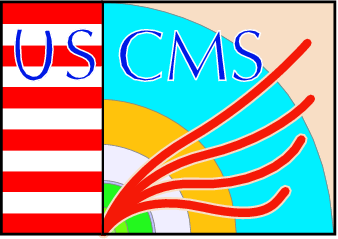
\includegraphics[height=0.6cm]{../../../Graphics/USCMS_logo.png}\hspace{.1cm}
\includegraphics[height=0.75cm]{../../../Graphics/UW_logo.png}}

\begin{document}

\begin{frame}
    \titlepage
\end{frame}

\section{Overview}
\begin{frame}
    \tableofcontents
\begin{itemize}
	\item OSG Storage Forum held at FNAL from 30 June to 01 July
	\item Agenda: \url{http://indico.fnal.gov/conferenceOtherViews.py?view=standard&confId=2538}
\end{itemize}
\end{frame}

\begin{frame}
\frametitle{Goals for the year (F. W\"urthwein)}
\begin{itemize}
	\item Support LHC users doing real work, especially at Tier3s
	\item Make life easier for storage administrators
	\begin{itemize}
		\item Simplify deployment and upgrades
		\item Improve technical support for sites
	\end{itemize}
	\item Increase Tier2 scale
	\begin{itemize}
		\item O(1M) files, 200-600 TB, 10-100 Hz to SRM via WAN, 1k-10k cores
		\item Limit maintenance cost to $<$ 0.5 FTE
	\end{itemize}
	\item Improve storage reliability at the Tier2s
	\begin{itemize}
		\item 80\% success rate in STEP09; 90\% of job failures due to LAN read errors
		\item Inadequate provisions for replication/redundancy at Tier2s
	\end{itemize}
\end{itemize}
\end{frame}

\section{Storage Technologies}

\subsection{dCache}
% monitoring (health check, stuck, absent, usage)

\begin{frame}
\frametitle{Development News and Plans (T. Perelmutov)}
\begin{itemize}
	\item SRM performance improvements
	\item All logging goes through Log4j!
	\item New pool code (better space accounting, migration of files between pools, fast startup and lower memory usage)
	\item XML info service: \url{http://${ADMIN\_NODE}:2288/info}
	\item Time-based release schedule
	\begin{itemize}
		\item 1.9.4: 20 July
		\item 1.9.5: after 1.9.4\ldots{} (used for first round of data taking)
	\end{itemize}
	\item Chimera replaces PNFS, but PNFS will be supported until all sites have migrated
	\begin{itemize}
		\item Not specific to PostgreSQL; will run on any JDBC enabled database (including Oracle)
		\item Use SQL to answer common administration questions, native database tools for backup
		\item Migration of a `normal' Tier2 should take less than a day
	\end{itemize}
\end{itemize}
\end{frame}

\begin{frame}
\frametitle{From PNFS to Chimera (F. Hu)}
\begin{itemize}
	\item Lots of limitations and problems with PNFS; no longer actively developed
	\item Chimera is the next generation namespace provider for dCache
	\item Database driven, scalable
	\item Instructions: \url{http://trac.dcache.org/projects/dcache/wiki/ChimeraSetup}
	\begin{itemize}
		\item Namespace must be migrated from PNFS to Chimera (requires downtime)
	\end{itemize}
	\item Purdue tests show Chimera scales well (and much better than PNFS with either DBD or PostgreSQL backends)
\end{itemize}
\end{frame}

\begin{frame}
\frametitle{Replication}
\begin{itemize}
	\item pcache (C. Waldman)
	\begin{itemize}
		\item Hardlinks files (PNFSID to LFN), providing fast access to files already stored on disk
		\item In use at some ATLAS sites (MWT2/University of Chicago)
	\end{itemize}
	\item {\tt billingrep} (W. Maier)
	\begin{itemize}
		\item \url{http://code.hep.wisc.edu/dcache-tools}
		\item Fast, first-order replication of files as they're written (within seconds)
		\item Complements the PFM
		\item Watches billing log for new files and runs {\tt pp get file} on a random pool
		\item Doesn't know about replicas that become unavailable (that's PFM's job)
		\item Allows PFM to run at a leisurely pace while keeping files (relatively) safe
	\end{itemize}
\end{itemize}
\end{frame}

% site talks
% development plans
\subsection{Hadoop}
% scalability of bestman+hadoop
\subsection{Lustre}
\subsection{Xrootd}

\section{Storage in the OSG}
\subsection{Information Services}
% gip, GLUE/search tool
\subsection{Packaging}
% toolkit, VDT

\end{document}
